\chapter{Functional Schema}\label{Functional_Schema}

\section{Datapath}\label{datapathch}

\begin{figure}
    \centering
    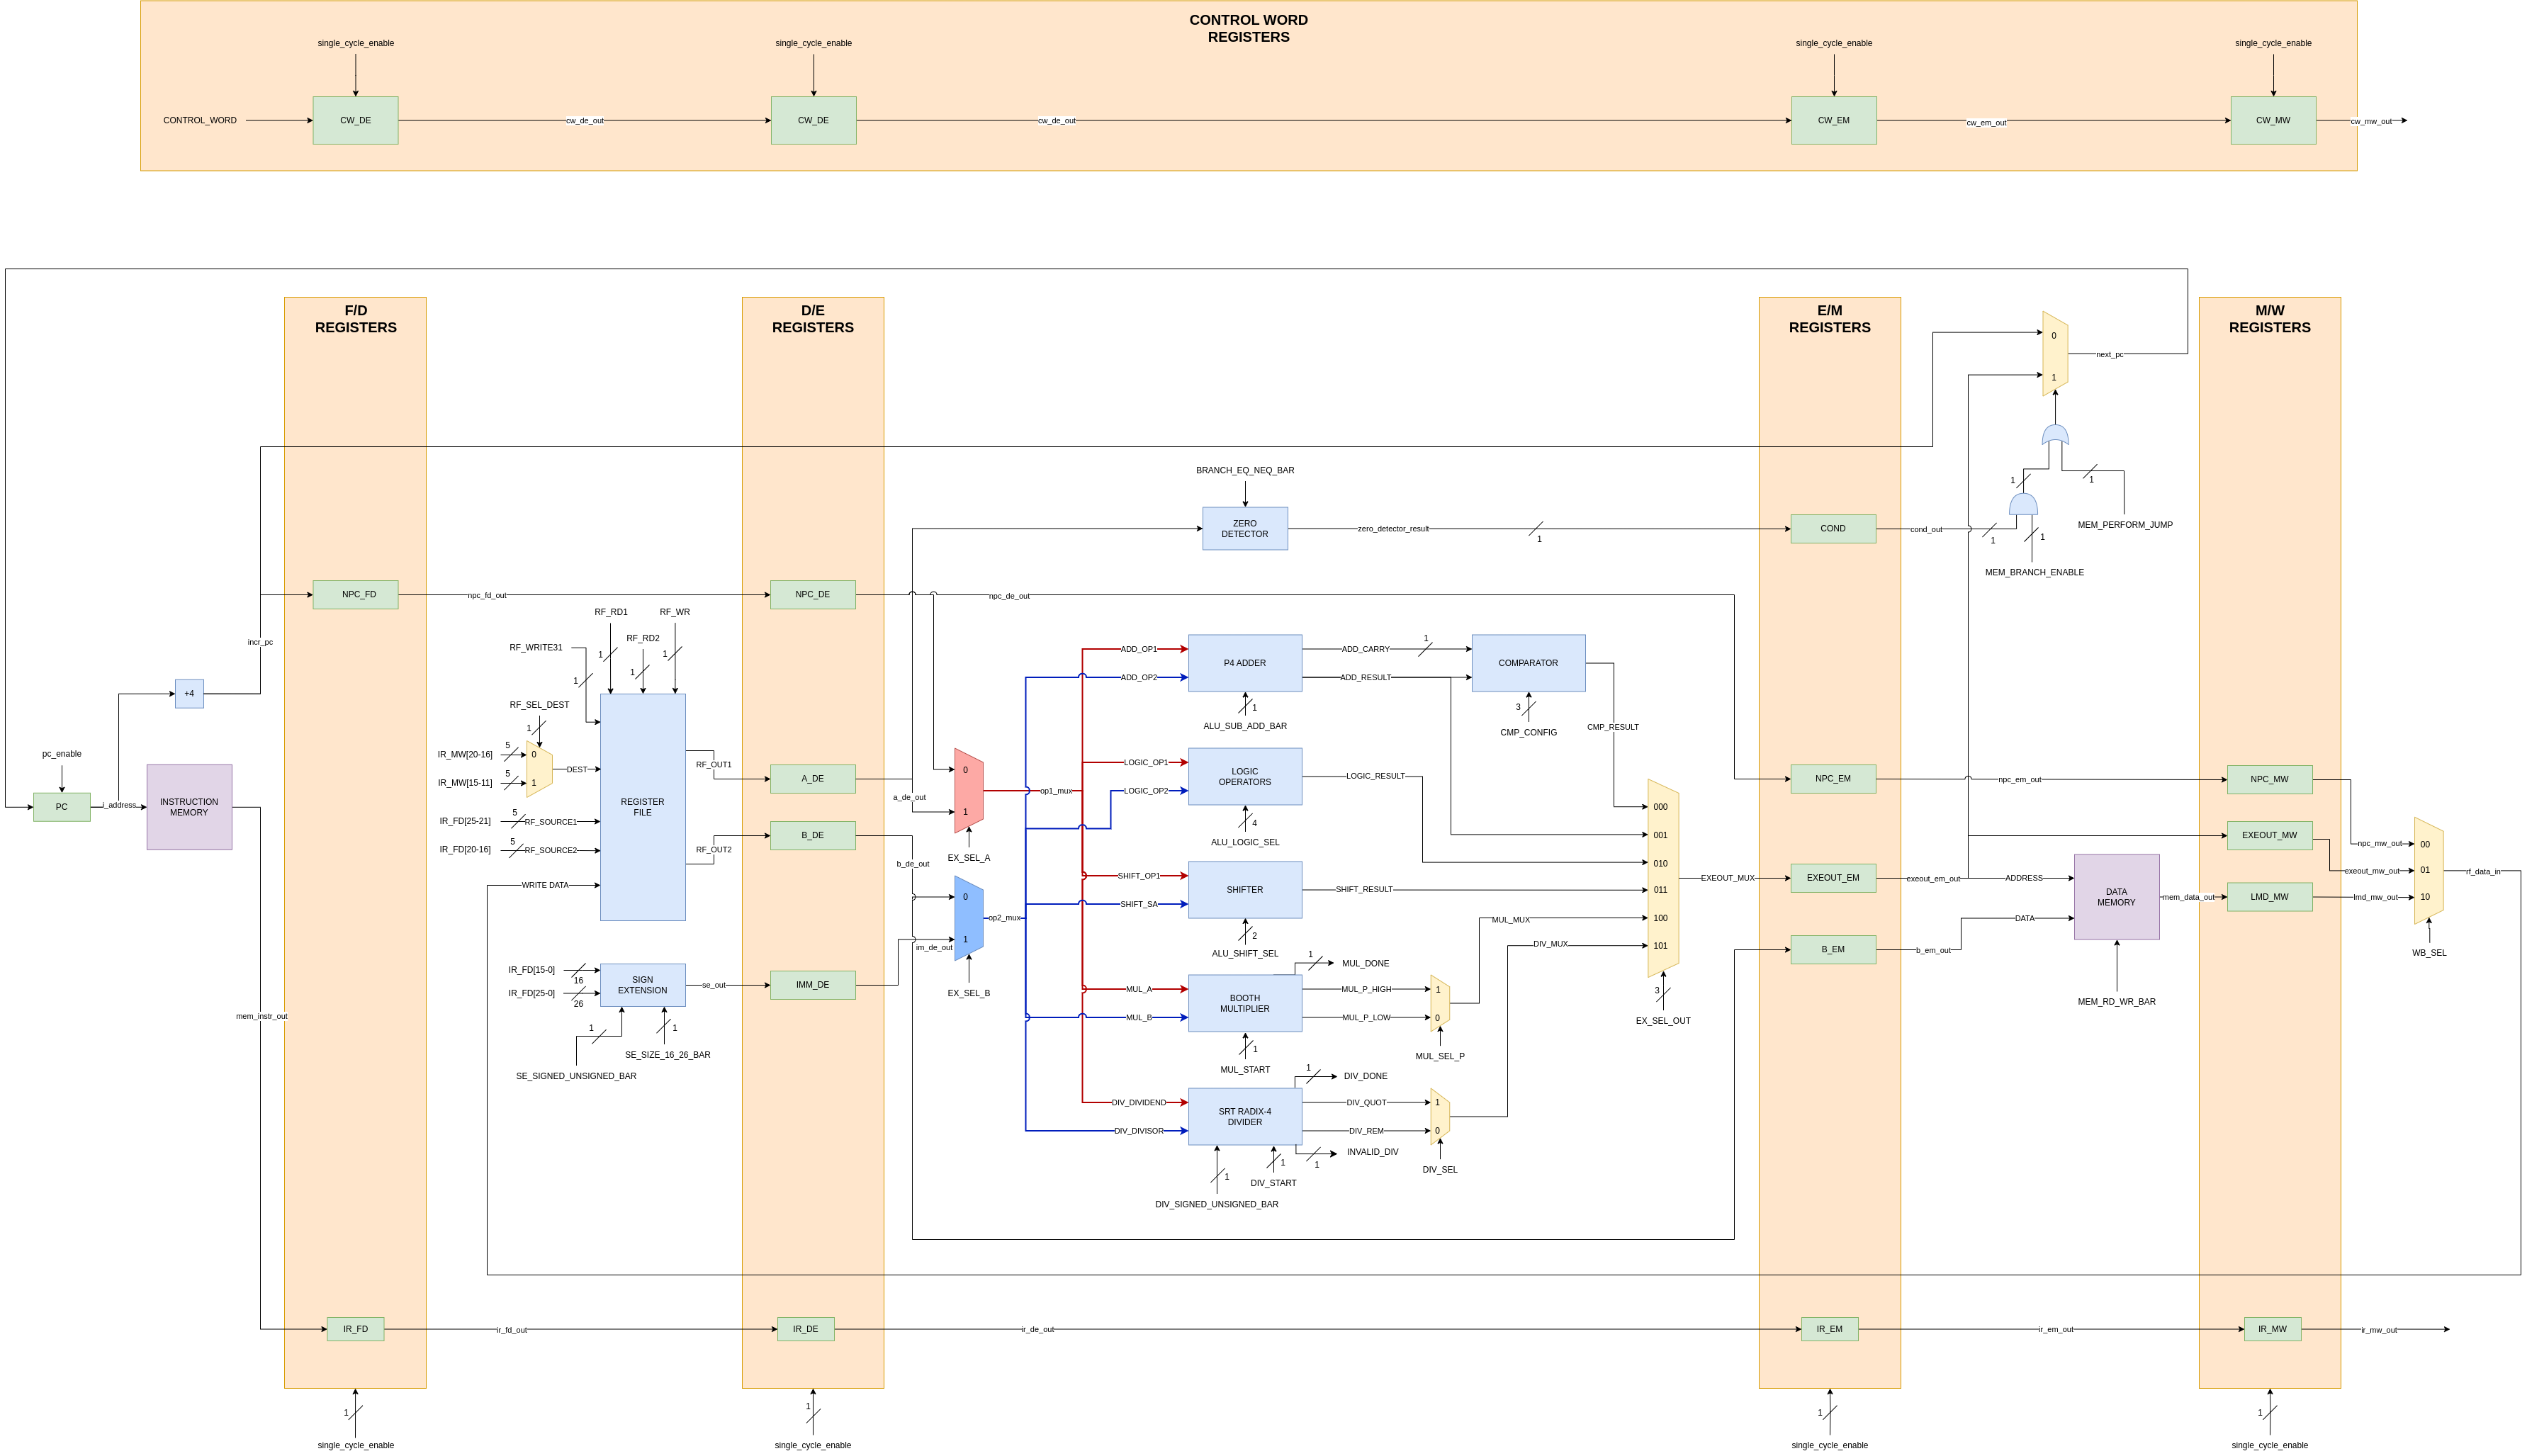
\includegraphics[width=1.4\linewidth, angle=-90, origin=c]{images/datapath.png}
    \caption{Datapath diagram}
    \label{fig:datapath}
\end{figure}

The full picture of the datapath of out DLX can be seen in \autoref{fig:datapath}; tt can be found in high quality inside \texttt{doc/diagrams} folder.
In this section we are going to cover the interconnection between the different components of the various stages of the pipeline, highlighting some implementation choices.
A full overview of the components can be found in \autoref{components_overview}.

\subsection{Fetch stage}

During the fetch stage (shown in \autoref{fig:fetch_stage}), the address stored in the program counter (or \textit{PC}) is used to access the instruction memory and read the next instruction to be executed.
Although in the diagram the instruction memory is shown as if it were part of the datapath, it is external and the same holds for the dram. 

The fetched instruction is stored in the \texttt{IR\_FD} register; the \texttt{IR} registers of the pipeline are in charge of moving the instruction that is being executed through the stages, so that it can be used if needed (for example to know the destination register).

In the meantime, the controller receives only the opcode of the fetched instruction and it generates the control word that will be used.
The control word is stored in the \texttt{CW\_FD} register, so that it will be available in the next stage of the pipeline. 
The control word then flows through the \texttt{CW} registers: only the signals needed for the following stages are propagated.

The next program counter (so $PC + 4$) is saved in the \texttt{NPC\_FD} register and will be propagated as well in order to be available for use in the next stages.

The program counter's content is written during the memory stage: it can be either the next program counter or another address computed during a jump/branch instruction. 
Th PC's value is updated only if the \texttt{PC\_enable} signal is one, otherwise it keeps its old value. 
This is useful for multi-cycle instructions, during which the pipeline has to stop. 

For the same reason, all the registers of the pipeline are enabled by the \texttt{single\_cycle\_enable} signal, so that they do not update during the execution stage of a multi-cycle instruction.

\subsection{Decode stage}

During the decode stage, all the possible operands for the execution stage are produced.
At this moment, we do not know which operands are going to be needed: they could both come from the register file, one could be an immediate and the other might come from the register file, etc.

We use \texttt{IR\_FD[25:21]} and \texttt{IR\_FD[20:16]} as read addresses for the register file. 
The read values are accessed through the \texttt{RF\_OUT1} and \texttt{RF\_OUT2} lines, and stored in the \texttt{A\_DE} and \texttt{B\_DE} registers.
Read operations on the register file are performed only if the control signals \texttt{RF\_RD1} and \texttt{RF\_RD2} are one. 

In the meantime, the sign extender produces the extension of the immediate value that may be used in the following stage. 
If we are dealing with an \textit{I-type} instruction, the immediate is located in \texttt{IR\_FD[15:0]}, and it will be extended as signed or unsigned number depending on the value of the control signal \texttt{se\_signed\_unsigned\_bar} (it's sign-extended during arithmetic operations, and zero-extended during logic operations); in case of a \textit{J-type}, the immediate is in \texttt{RF\_ID[25:0]} and is always sign-extended.
The extended immediate is stored in \texttt{IMM\_DE}.

\begin{figure}
\centering
\begin{minipage}{.5\textwidth}
  \centering
  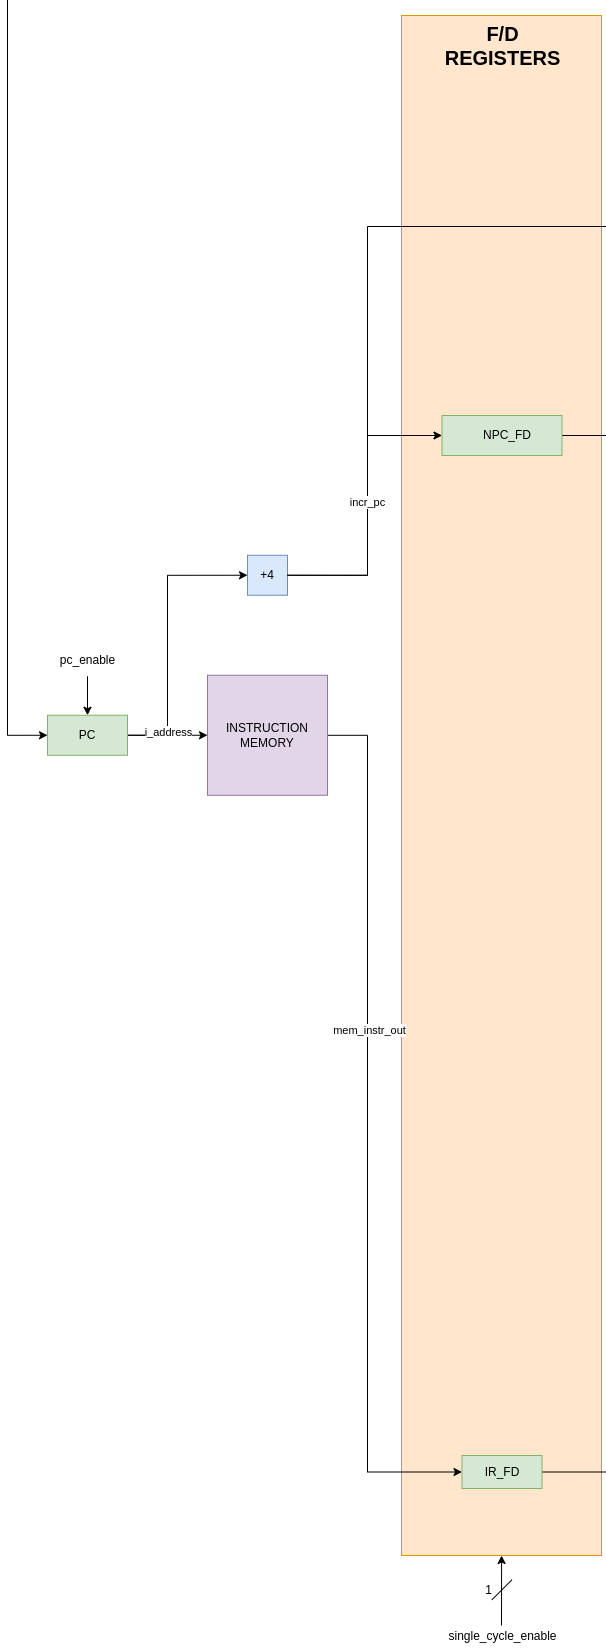
\includegraphics[height=1.80\linewidth]{images/fetch_stage.png}
  \captionof{figure}{Fetch stage of the datapath}
  \label{fig:fetch_stage}
\end{minipage}%
\begin{minipage}{.5\textwidth}
  \centering
  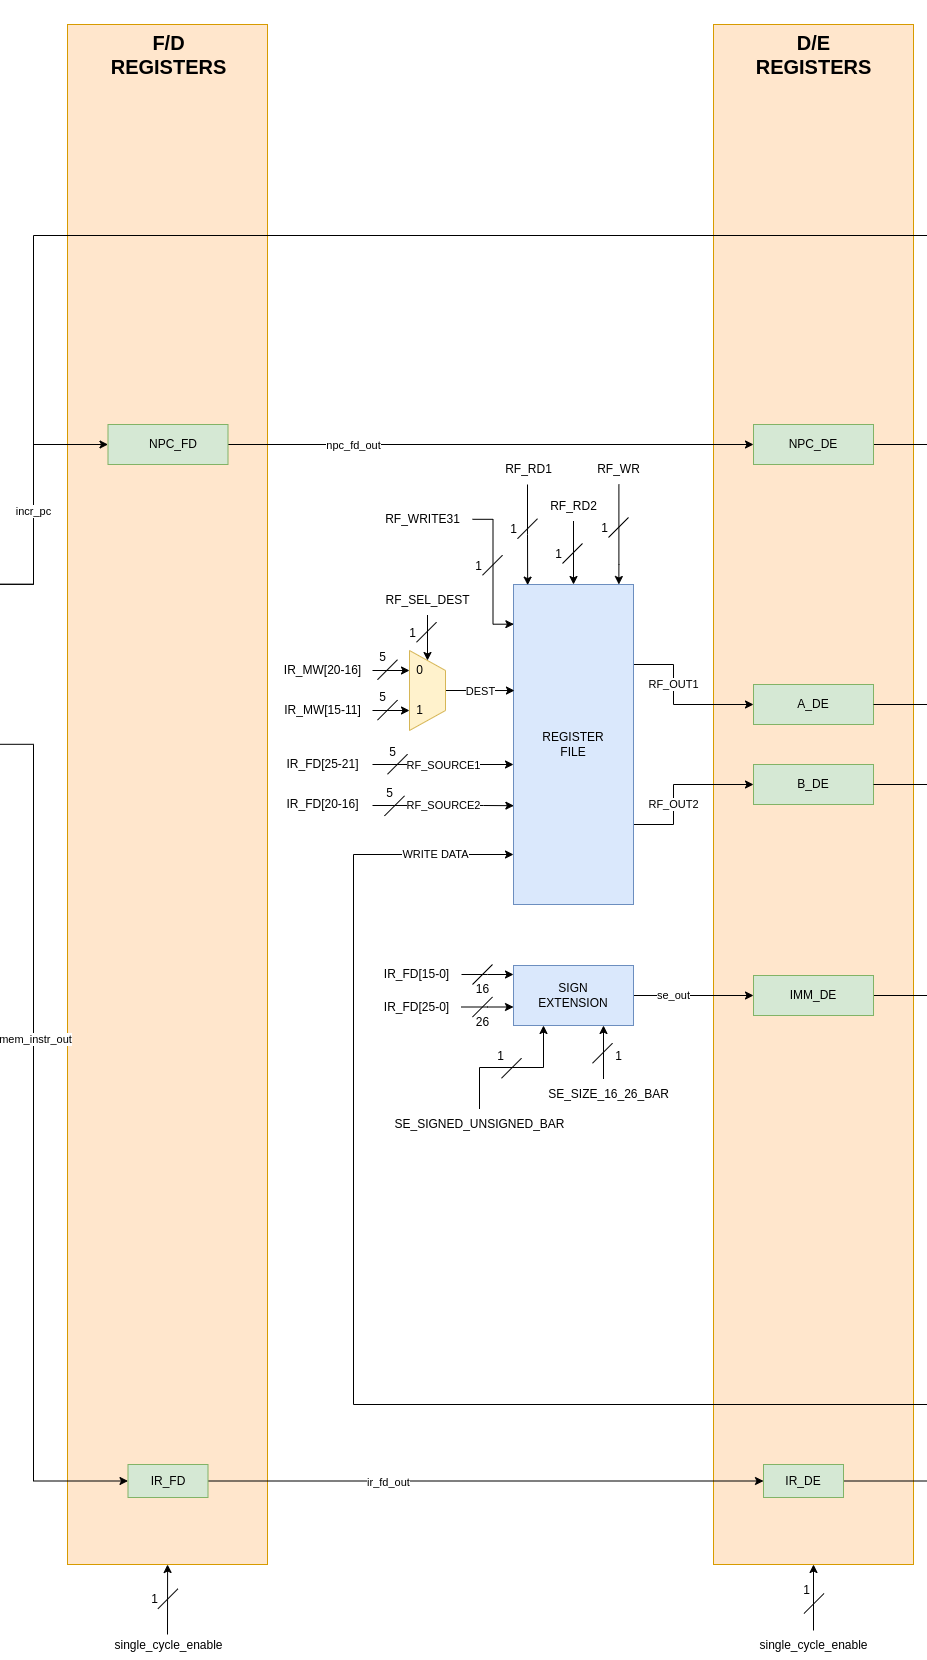
\includegraphics[height=1.80\linewidth]{images/decode_stage.png}
  \captionof{figure}{Decode stage of the datapath}
  \label{fig:decode_stage}
\end{minipage}
\end{figure}

\subsection{Execute stage}

In the execution stage, shown in \autoref{fig:execute_stage}, the operands are used to perform an operation using one of the available components.

The first two multiplexer decide which will be the operands, according to the control signals \texttt{EX\_SEL\_A} and \texttt{EX\_SEL\_B}. 
When \texttt{EX\_SEL\_A} is one, the first operand is the one read from the first port of the register file, otherwise it is the next program counter, computed during the fetch stage of the same instruction that is now in the execution stage.
When \texttt{EX\_SEL\_B} is one, the second operand is the previously extended immediate, otherwise is the one read from the second port of the register file.

The possible operations that can be performed are: addition, subtraction, shift (left or right, arithmetic or logical), logical operations (or, nor, and, nand, xor, xnor), multiplication or division. 

In case a multiplication or a division starts, the pipeline is stopped until a finish signal is raised: should that happen, the controller will resume the pipeline after one clock cycle.

In case of a division, the possible output can be either the quotient or the remainder.
Regarding the multiplication, we are multiplying two 32-bit numbers, so the result is 64 bits: for this reason, you can select either the upper part of the result (so its 32 MSBs) or the lower part (so its 32 LSBs).

The result of a subtraction is also used to compare the two inputs using a comparator. 
According to the \texttt{CMP\_CONFIG} signals, the result is one if the requested comparison is true, otherwise it is zero.
This component is often used to compute a condition based on which a branch might or might not be performed.

The signal to be sent as output is chosen thanks to the last multiplixer, driven by the \texttt{EX\_SEL\_OUT} signal.
Both the next program counter and the B operand are also propagated through the pipeline, since they will be used in the following stage. 

The value of the register \texttt{A\_DE} is also used to check the condition of a branch using the zero detector. 
The output of this component is one if the operand is zero and we are performing a \texttt{beqz} operation or if the operand is not zero and we are performing a \texttt{bnez} operation (in these cases the branch is taken); in all other cases it is zero (meaning that the branch is not taken). 

\begin{figure}
    \centering
    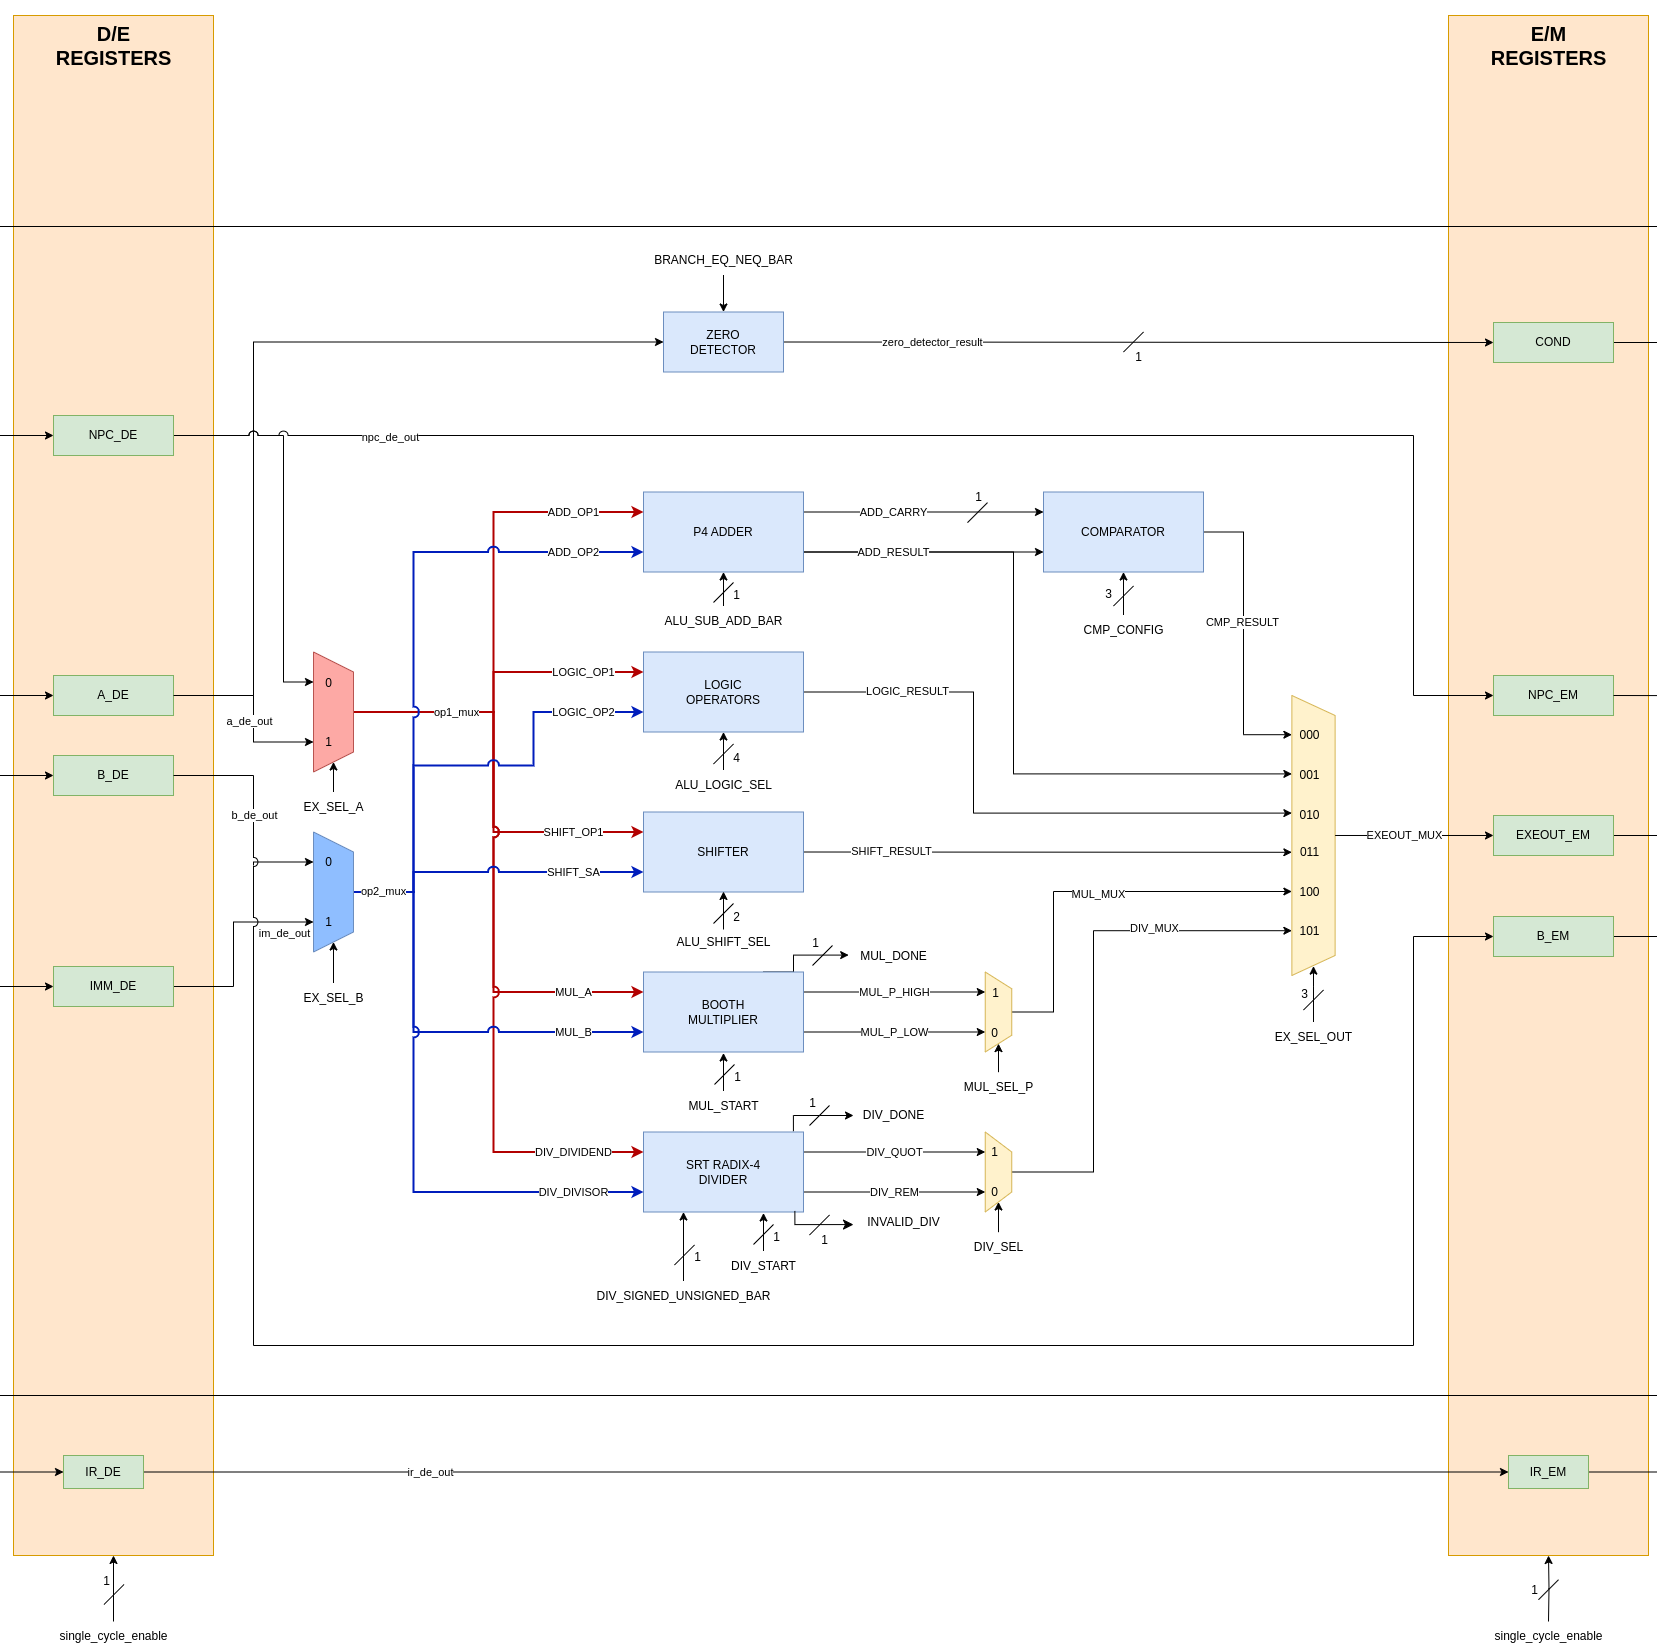
\includegraphics[width=1\linewidth]{images/execute_stage.png}
    \caption{Execute stage in the datapath}
    \label{fig:execute_stage}
\end{figure}

\subsection{Memory stage}

The memory stage shown in \autoref{fig:memory_stage} is used both to access the dram (in case of a load/store operation) and to compute the next value of the program counter. 

The new program counter is:
\begin{itemize}
    \item $PC + 4 + immediate$ if we are performing a branch and the condition is true (the immediate value stored inside the instruction is an offset relative to $PC + 4$);
    \item $PC + 4 + immediate$ if we are performing a jump or a jump-and-link;
    \item the value read from a target register if we are executing a \texttt{ret} instruction;
    \item $PC + 4$ in all the other cases.
\end{itemize}

If we need to perform a read operation from the dram, the signal \texttt{mem\_rd\_wr\_bar} is one, otherwise it is zero.
The address is computed in the execution stage by adding the content of a register with the immediate value in the instruction. 
The value to be written is stored inside \texttt{B\_EM}; the read value is stored into \texttt{LMD\_MW}. 

\subsection{Write back stage}

In the write back stage, as shown in \autoref{fig:writeback_stage}, we write to one register in the register file in case the \texttt{RF\_WR} signal is one. 
The destination register is located in \texttt{IR\_MW[20:16]} or in \texttt{IR\_MW[15:11]}, depending on the type of the instruction.

The value to be written can be:
\begin{itemize}
    \item $PC + 4$, in case of a jump-and-link instruction;
    \item the value read from the memory, in case of a load instruction;
    \item the result of the execution stage, in all the other cases.
\end{itemize}

The register file is configured to perform the writing operation on the falling edge of the clock (technically it writes on the rising edge of the negated clock, since the tech library used doesn't include negative-edge triggered flip-flops). 
This decision might decrease the overall performance from a delay point of view (by increasing the critical path) but it allows the processor to write and read data from the same destination in the same clock cycle, thus reducing the latency of data-dependent instructions by one clock cycle.
In this way, each time there is a RAW dependency between two instructions, there must be only two instructions to separate them, not three. 

Since in a \texttt{JAL} instruction the destination is implicit (\texttt{r31}), the register file has a \texttt{RF\_WRITE31} signal which forces the write destination to the thirty-second register if it is one.

\begin{figure}
\centering
\begin{minipage}{.5\textwidth}
  \centering
  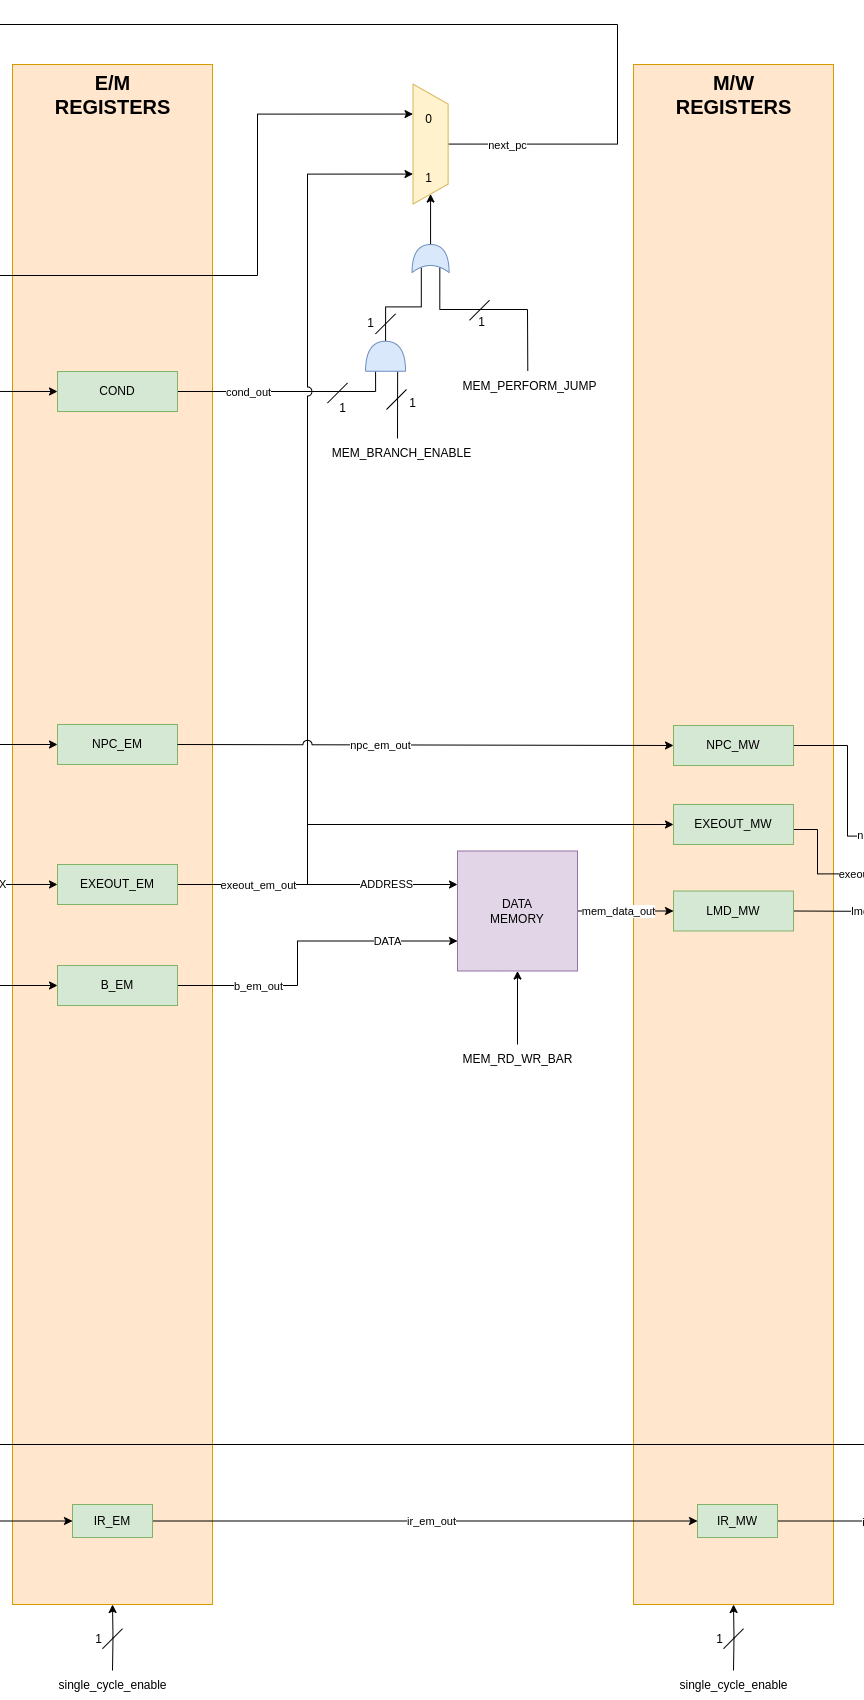
\includegraphics[height=1.80\linewidth]{images/memory_stage.png}
  \captionof{figure}{Memory stage of the datapath}
  \label{fig:memory_stage}
\end{minipage}%
\begin{minipage}{.5\textwidth}
  \centering
  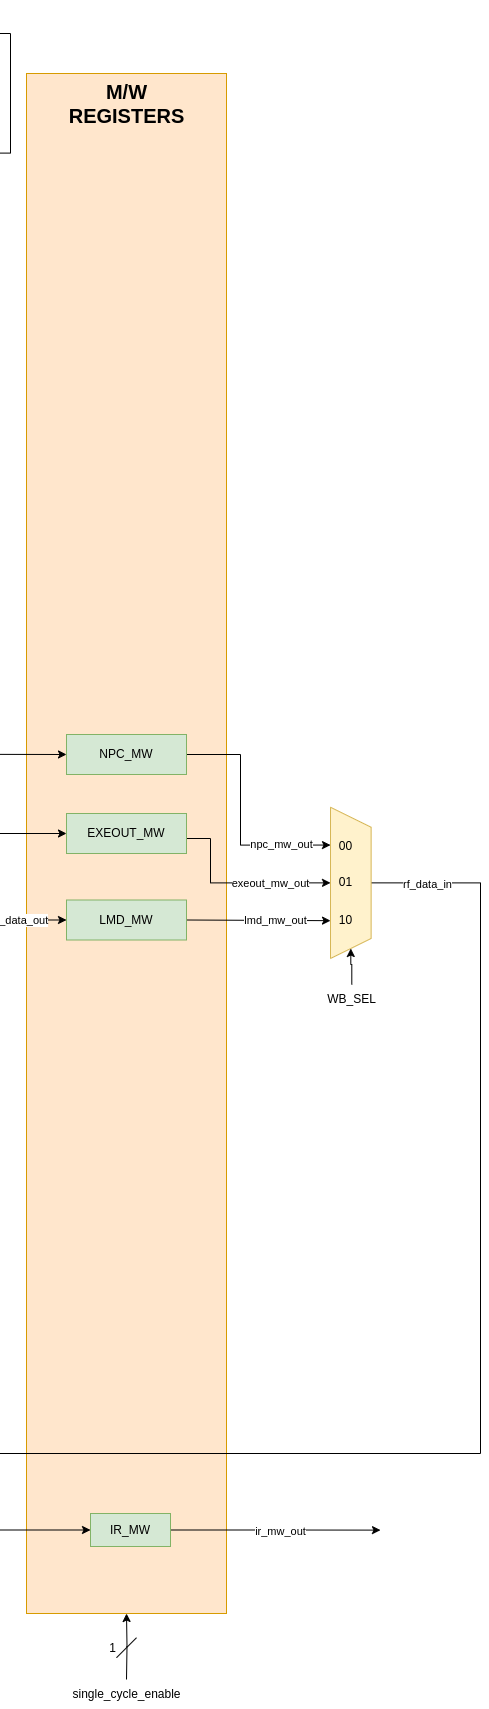
\includegraphics[height=1.80\linewidth]{images/writeback_stage.png}
  \captionof{figure}{Write back stage of the datapath}
  \label{fig:writeback_stage}
\end{minipage}
\end{figure}

\section{Controller}\label{controller_ch}

The control unit of the processor communicates directly with the datapath unit and generates the necessary commands to guarantee its correct behaviour and the execution of its nominal functions. 

A hybrid FSM-hardwired controller has been used in our processor, as it is the most convenient choice in the presence of a pipelined datapath with support for multi-cycle operations. 
The management of the pipeline is made possible by a series of registers, so that every stage receives the correct control word at each clock cycle.  

The controller receives as data inputs the opcode coming from the instruction memory and some status signals from the high-latency components (divider and multiplier), while it outputs the control word associated with the received opcode and the enable signals of some registers.
A look-up table is used to store all the control words and is addressed using the instructions' opcodes. 
The controller's FSM has two possible states (or modes): \textit{single-cycle} and \textit{multi-cycle}.

In single-cycle mode the control word is generated combinationally and according to the opcode received from the IRAM, so the controller behaves like a hardwired control unit. 
If the opcode of a multiplication or a division is recognised, then the controller will stop the instruction fetching after one clock cycle (by disabling the program counter) and will wait another clock cycle before switching to multi-cycle mode: during this time period it doesn't stop the control word generation.
This latency before changing state is necessary to guarantee that the controller is in multi-cycle mode when the high-latency operation is in the execution stage.

In the multi-cycle state the controller stops generating the control words and disables the control word registers and the registers between the stages, effectively halting the pipeline: this is done to allow the multiplication/division components to complete their operations.
Once this happens, the high-latency component in use will raise an "operation complete" signal: once that happens the controller will go back to single-cycle mode after one clock cycle, thus allowing the pipeline to resume its operations.

It is important to know that the controller can manage only one multi-cycle instruction at a time: details on how different situations are given in \autoref{dependencies}.